\documentclass[11pt,twocolumn]{article}
\usepackage[utf8]{inputenc}
\usepackage{graphicx}



\graphicspath{}

\author{
  \texttt{Sebastian Bångerius}
  \and
  \texttt{Villiam Rydfalk}
}

\begin{document}
\pagenumbering{gobble}

\title{Multi-path throughput in mobile networks}
\maketitle

\cleardoublepage


\section{Abstract}

In this project we evaluate and make some conclusions about the use and efficiency of TCP with multipathing. This is a new protocol in progress often referred to as MPTCP. We will only have data from an LTE network, but will discuss the use of this in other networks as it is a strength of the protocol to use many paths, possibly over many different types of networks. We aspired to do our own simulations, but as the time was short and the programs we found  were too complex and our knowledge of coding C++ was limited we could not complete any of our goals. We will include a discussion of our, even though limited, experience with these simulators as well as the strengths and weaknesses of both them both. So instead of using our own simulations as grounds we had to use results of another study. \cite{MPTCP-LTE} We analysed the results we made some hypotheses about what we were expecting. Once we've analysed their method and looked over their results we made our own conclusions and posed a few new questions that would be interesting to investigate in further studies.


%We have made a project about the throughput in multipath networks. Specifically in WiFi and Bluetooth networks. By analysing and comparing these we have made a few conclusions about strengths and weaknesses for both. We have done a simulation of some scenarios based on the real world and what might happen in a network. We had some hypothesis about what should happen in these scenarios and discussed possible solutions. Once we conducted the simulations we revised our hypothesis and made an analysis of the results. We came to a conclusion and discussed other possible scenarios. We have also made some hypothesises about when and where the different methods of network routing should be used and a few examples of implementations.%

\section{Introduction}

The way we transfer information varies a lot between places and situations. Some techniques work better in certain environments, while they encounter complications in others. People in different countries have different interests, standards and financial potential. Because of all these circumstances affecting mobile networks, it is important to actually study how information flows through them. For instance; in areas with high population density there might be easier to rout data between end users towards an access point, while in sparsely populated areas it might be better with one cellular tower (or even a satellite) for connection. In a lot of central and southern African countries people have access to a phone but no electricity, in such an environment power saving might be a key feature of data transfer, and some power consuming routing options are excluded.

Even though it is old, TCP is the most widely used protocol for data transferring. But with a growing internet and the number of users rising extremely fast the need for a more effective service is needed. Specifically with mobile devices like phones that use many different types of networks there is a lot of potential for improvement. They can establish connections to the Internet via various interfaces such as 3G, WiFi, LTF and Bluetooth. The implementation of TCP over multiple channels is something that was discussed during the 10th International IFIP TC 6 Networking conference in Valencia in 2011 \cite{RFC6824}. It was argued that as our devices have so many different interfaces we need to update the original protocol that was introduced when we used only one interface for the transport layer in the protocol stack. And multiple channels for utilization is something we hope to be able to at least argue for and make a few assumptions about it in the end.


%There are many ways to transfer information electronically, however in this report we will focus on routing in different kinds of networks and different methods of routing. In many networks there is a lot of data flowing and the traffic is very high over certain paths. If a path is faster than other then many protocols will try to use that path even though it is heavily burdened since it is hard to measure traffic until after a packet has failed to be delivered. So one way to solve this is by sending a few packets over a different path even though it is slower. This is referred to as multipathing. The theory is that by sending packets different routes the throughput and effective use of the network will be higher than if the devices send all packets the same route. 

\section{MPTCP}
The Internet Engineering Task Force (IETF) is working on MPTCP. RFC 6824 is experimental and has been in progress since January 2013. It is well worked out and is not far from being ready for being put to industrial use. But as such there is no real implementation of it outside the experimental phase, so there are no finished simulators or modules of MPTCP yet. There are a few studies made outside IETF built on what the RFC has stated and they have made some simulations that are publicly available, but they are not easily implemented unless a lot of work is put down.

MPTCP uses the same method for sending and receiving packets as TCP. The difference is that it can do so with multiple connections simultaneously. If both the client and server have several addresses linked to it they can set up several connections between themselves using a different address for each connection. These extra connections are usually called additional subflow setup, in contrast to the initial connection setup. MPTCP identifies multiple addresses and for each pair it sets up a connection. Each of these connections then works as a normal TCP connection starting with the normal syn, syn-ack and ack as handshake and it uses the same method of congestion control as normal TCP.

MPTCP is also supposed to be able to open subflows on different TCP-ports. The benefits of this  aren't as obvious as in the previously mentioned scenario (of different network addresses) as chances are the packets will end up on the same route anyway. 

\section{Method}

We want to evaluate different methods of pathing in a network to get good throughput. If we are to do any tests on a larger scale it will be a lot of complex work unless we do a simulation. But since we didn't manage to get any of the simulation programs working, we will use the results of another articles work. The article called \emph{Multipath TCP in LTE Networks} and in it they have results from simulations we would have wanted to do so by using their results we will probably be able to draw the same conclusions we would have with our own simulation, if not even better.

The method they used was to set up a network with a data flow program called Iperf. They then used a program called tcptrace to get the information about transmission speed, delay and other various details about the connection and transmission. This was then processed in a data analysis tool called UDA. We have not used, nor heard of any of these tools previously, but we mention them as it might be a good idea to have them in mind when looking at the result and if we are to do further studies of our own.

%First of all we need a few nodes that can connect in a way we want, and they have to be able to communicate with a given quantity of data that we can measure. We also need to be able to split this data up in any way we want between several paths. In these paths we have to be able to set different factors like noise, other traffic and just about anything that would interfere with our packets in a "real world" scenario.

%Once we have software that can do all this we have a few experiments we will try. At first we will just test the most simple networks with only a few nodes sending data to each other without any real interference to get a sense of what is good throughput and a calm network. Once we have done this we will raise the complexity of the network. Add more nodes that communicate with each other and flooding the network with packets. Our hope is to be able to do this as gradually as possible to see the decline in effectiveness of the network. Hopefully we will be able to see a trend of what factors do the most good or harm to the network and what methods of routing are best for each different scenario.

The specific scenario they used was a server with two ethernet interfaces conected to the Internet with a lot of capacity. The client has two LTE modems that connects it to the internet. MPTCP was then set up using all different combinations of connections, so a total of 4 different connections. See figure 2.
 
\begin{figure}[ht]
\begin{center}
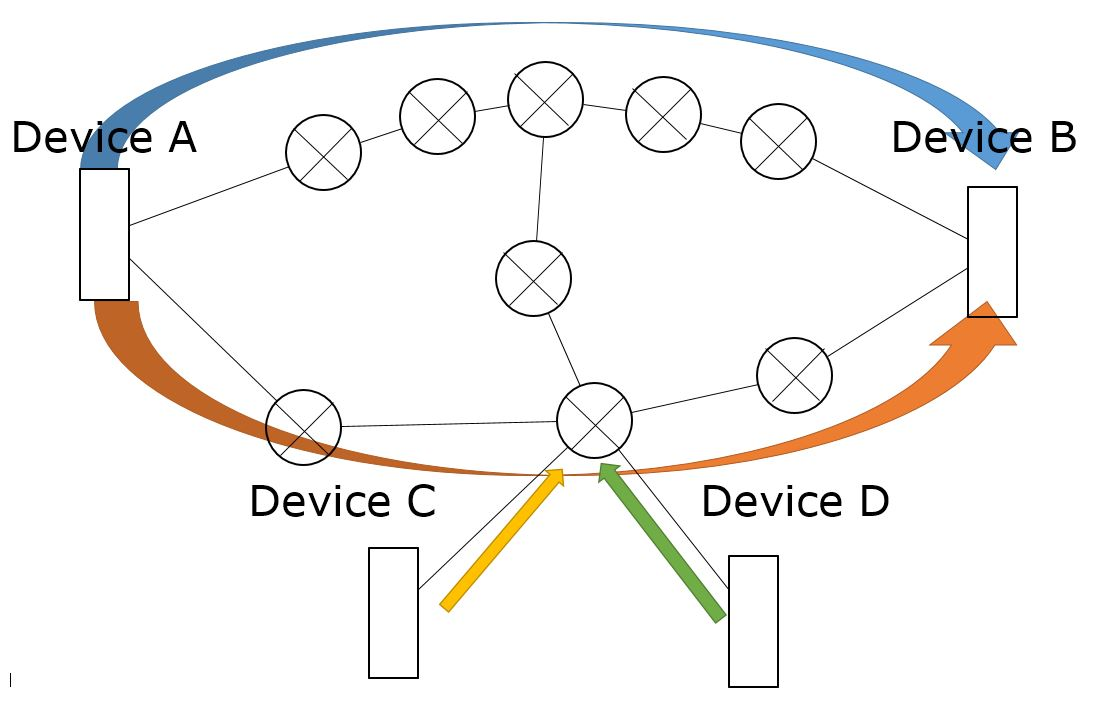
\includegraphics[scale=0.26]{Figure_1}
\end{center}
\end{figure}

In addition, they did make the connections a bit different. The two LTE interfaces have different quality and power. LTE0 has slightly lower power but higher quality than LTE1. We wont go into detail about these two mesurements of power and quality, but they are referred to as Reference Signal Recieved Power and Reference Signal Recieved Quality, or for short RSRP and RSRQ.


\section{Hypothesis}

When it comes to networks in the real world there will be a lot of different types and some won't have the same problems as others. But in ad-hoc networks where there is a lot of information to be sent between the nodes there will be a lot of traffic, and a lot of burdening on some paths since there will always be one path that is faster than another.

Even though MPTCP has some drawbacks, including: Higher power usage, resources used to manage the cooperation of the connected interfaces and increased complexity, we still believe that it will produce great throughput performance that in some scenarios will be preferred over (for instance) power consumption.

With the test we are going to do evaluate weather multipathing helps a network to get a higher throughput or not. Our guess is that it will improve the performance of the network and here is why:

When a path is used very heavily then the traffic there might collide and cause dropped packets. This will result in delays and more traffic back and forth. This could be avoided if the nodes were to use 2 or 3 of the fastest routes instead of just the single fastest one. If the network is not very burdened then this might be a waste of time since it might take longer for the data to arrive than if it sent all over the same fast path, but in a network with a lot of users and a lot of traffic it might improve the chance of a stable line of communication.

Also, when there is a lot of different paths there is less chance of trouble if one path would be broken since you already have a few other paths saved. If you simply used one path you would now have to search for a new one before being able to send the rest of your data.

There are still some problems with multipathing. When looking at multipathing between cellular and Wifi (which is probably the most relevant multi-channel implementation) we can often see a significant difference in RTT (round trip time). We believe that this might end up showing some interesting effects in the case of multipathing. We also often have the issue of the cellular connection being metered, which is a strong reason to not use it if wi-fi is available. These two facts lead us to believe that there are ways to use the multipathing so that both links are able to bring their respective benefits into the multipathing algorithms. One might be able to distribute the data over the two links depending on some attribute of the data, for instance how big the packet is or what application requested the TCP-delivery. Though the latter suggestion will probably violate the protocol stack praxis.

\section{Results}

\emph{Note: We will use the tables and graphs of the original report\cite{MPTCP-LTE} in this segment. All tables and graphs can be found in that report. We use them only as a means of discussion.} \\

The goal of the tests were to verify the efficiency of MPTCP in an LTE mobile network environment. There were three separate tests done. The first simulation was a TCP connection over a single path where they test the throughput and RTT to have something to compare with. The results were as follows in figure 2 and figure 4.

\begin{figure}[ht]
\begin{center}
\includegraphics[scale=0.6]{table_1}
\caption{Result table of test 1}
\end{center}
\end{figure}
\begin{figure}[ht]
\begin{center}
\includegraphics[scale=0.5]{graph_1}
\caption{Result graph of test 1}
\end{center}
\end{figure}

This test shows the maximum throughput without MPTCP. As we do not have data of other types of networks or any experiance with testing other types of networks, this will only be used for comparison. In the source they make some statements about the results confirms the behaviour of LTE networks as they are supposed to have lower delays than, for example, EDGE. 

In the second experiment the MPTCP protocol was used, which generated very different results. We can verify that the channel 0 had a worse signal than channel 1, but managed to maintain a relatively high throughput even though the RTT was high. So if we compare figure 3 and 6 we can see clearly that the MPTCP has a much higher total throughput than a single path TCP connection.

\begin{figure}[ht]
\begin{center}
\includegraphics[scale=0.6]{table_2}
\caption{Result table of test 2}
\end{center}
\end{figure}
\begin{figure}[ht]
\begin{center}
\includegraphics[scale=0.5]{graph_2}
\caption{Result graph of test 2}
\end{center}
\end{figure}
\begin{figure}[ht]
\begin{center}
\includegraphics[scale=0.5]{graph_3}
\caption{Result graph of test 2}
\end{center}
\end{figure}

The third test was done to see how well MPTCP recovered from a failure. In this test channel 1 was randomly disconnected twice. The numbers in this test are beyond our limited knowledge of LTE, so we will mainly use the graphs as a means of discussing the recovery speed and sustainability of MPTCP. See figure 6.

\begin{figure}[ht]
\begin{center}
\includegraphics[scale=0.6]{graph_4}
\caption{Result graph of test 3}
\end{center}
\end{figure}



%\section{Time plan}
%\begin{description}
%\item[Week 38]
%Acquire information about how packets flow through different network types. %Get a more detailed plan.
%\item[Week 39]
%Write ~2 pages. Find and learn tools for network simulation. Complete %milestone 2
%\item[Week 40]
%Write ~2 more pages (so ~4 in total). Make first trial simulations
%\item[Week 41]
%Write ~3 more pages (so ~7 in total). Make sharp simulation. Draw %onclusions. Make beautiful diagrams in Excel. Drool over said diagrams.
%\item[Week 42]
%Seminar and finish report
%\end{description}

\section{Discussion}

\subsection{MPTCP vs TCP}
It is fairly obvious that MPTCP had a better throughput than the single connection TCP. The total throughput of the single path TCP was around 3 Mbps while the total throughput of MPTCP was around 7. Almost the double. Even though this is a very small simulation it does show the main strength of MPTCP, the ability to use more of the available paths than normal TCP. If we were to add a larger network we would presume the results to be very similar, maybe even better if there are a higher number of possible paths. Since the normal TCP is restricted to one path it just cannot compete on that type of problems if there are multiple available paths. If there was additional traffic with the chance of congestion and a higher risk of dropped packets the MPTCP would also have an advantage as it can use paths less travelled and thus be more effective. So if all devices would use such a method the efficient use of a network would surely rise, and the throughput would hopefully be higher as a result. Of course this would mean there would be a more evenly spread of traffic on almost every path and thus make it more likely to have collisions on even a long path that wouldn't be used with normal TCP.

There are some problems with MPTCP of course. In a presentation by IETF there are some pointers to problems with MPTCP.\cite{IETF-Probs}. They show that in some cases MPTCP could penalize TCP users. While the bottleneck for MPTCP users is at the server the TCP users often get a bottleneck in their own network. This means that MPTCP users make TCP users less effective without gaining throughput. As we have hinted before MPTCP might even make it harder for other MPTCP users as it would mean that everyone in the network gets a lowered throughput since a single user might send data through several bottlenecks at once, and thus making it harder for everyone to get data through the network.

So in conclusion what we can say about MPTCP is that it would be a good upgrade if we can first take care of the problems that it would cause for already existing users.


\subsection{Simulator programs}

Even though we didn't manage to simulate the MPTCP we did get a good look on a few different simulation programs. In particular NS-3 and OMNeT++. These two programs are very different in many aspects and have strengths and weaknesses.

The first glaring difference is how easy they are to acquire. NS-3 doesn't have compatibility with Windows. There are a few very experimental tests with Eclipse and Visual Studio (IDE's that run on Windows) but neither of them worked for us, they either were to complicated to get working or they just crashed. So the only way we managed to run NS-3 was to get a virtual machine with Linux Ubuntu on it. We used Oracle VM VirtualBox to set up a Ubuntu device and then we installed NS-3 on that device. The problem then was that the installation and build of the program took very long time. Once we had the program ready to run we realised the complexity didn't end there. Without any extended experience with Ubuntu we had a hard time knowing how to add the right modules and where to add them. The tutorials were scarce and hard to follow. We eventually managed to get some example programs running, but they were small and not related to our ideas of simulations. What we found then via a forum was OMNeT++ that was runnable on Windows via an Eclipse based IDE. It took a fair bit of time to install as well, but not nearly as long as NS-3. Once set up, OMNeT++ had a lot of interesting demos and examples, including SCTP which has a few similarities with both TCP and even MPTCP as it has multihoming capabilities. But unlike MPTCP it requires several IP-addresses to use different paths. In retrospective, it would probably have been good to have used OMNeT++ from the start and maybe taken a different route of what to simulate. But it is always easy to be smart in retrospective.

So the biggest strength of OMNeT++ we found at first was of course the ease with which it was installed and used since it had a very nice graphical interface that we were familiar with. Another cool thing with OMNeT was that it included support for a lot of different cool modules and plugins, including a google earth plugin so you could simulate networks on maps so that you get simulations that are very realistic and easy to relate to. NS-3, in contrast, was purely console based and had a much harder to use system of modules. To make a animated simulation it took a lot of reading and testing. Nothing came easy. So OMNeT really took the prize in being easy to use.

What OMNeT++ lacks is the report results. To make measurements the user has to do the coding for themselves. In NS-3 this is a function that is more or less built in. There are of course a lot of differences that we have not touched as well. We did only get a brief look at them during a very intensive two weeks. But this might be a good pointer to the programs and a reminder that the tools used greatly affect the speed of which a project can be completed.

\newpage

\begin{thebibliography}{9}

\bibitem{MPTCP-LTE}
Ondrej VONDROUS , Peter MACEJKO , Zbynek KOCUR \\
\emph{Multipath TCP in LTE Networks}\\
Czech Technical University in Prague, 2014

\bibitem{VALENCIA}
BARRE, S., Ch. PAASCH and O. BONAVENTURE.\\
\emph{MultiPath TCP: From Theory to Practice.}\\
In: 10th International IFIP TC 6 Networking
Conference. Valencia: Springer, 2011

\bibitem{RFC6824}
RFC 6824.  \\
\emph{TCP Extensions for Multipath Operation with Multiple Addresses} \\ 
https://tools.ietf.org/html/rfc6824.\\ IETF, 2013.

\bibitem{IETF-Probs}
R. Khalili\\
\emph{Performance issues with MPTCP}\\
https://www.ietf.org/proceedings/84/slides/slides-84-mptcp-4.pdf



\bibitem{Comparison}
Murat Miran Köksal\\
\emph{A Survey of Network Simulators Supporting Wireless Networks} \\
October 22, 2008



\end{thebibliography}




\end{document}